%
% File naaclhlt2015.tex
%

\documentclass[11pt,letterpaper]{article}
\usepackage{naaclhlt2015}
\usepackage{times}
\usepackage{latexsym}
\usepackage{amsmath,amssymb}
%\usepackage{microtype}
\usepackage{graphicx}
\usepackage{rotating}
\setlength\titlebox{6.5cm}    % Expanding the titlebox

\title{An extendable, multilingual textual entailment engine by
  multi-level alignments} 

\author{Author 1\\
	    XYZ Company\\
	    111 Anywhere Street\\
	    Mytown, NY 10000, USA\\
	    {\tt author1@xyz.org}
	  \And
	Author 2\\
  	ABC University\\
  	900 Main Street\\
  	Ourcity, PQ, Canada A1A 1T2\\
  {\tt author2@abc.ca}}

\date{}

\begin{document}
\maketitle
\begin{abstract}
 abstract text 
\end{abstract}

\section{Introduction}
One key challenge at the core of Natural Language Processing (NLP) is
the ability to determine which conclusions can be inferred from a
given natural language text. An engine that answers this problem,
recognition of Textual Entailment (TE), has the potential to become
the generic semantic processing engine for various NLP tasks.    

TE technology has matured over the last decade. TE modules are being
utilized in various semantic applications, and researchers can find a
range of well developed algorithms, methods and even software suites. 
With various possible choice of open source engines, it is now much
easier for new users to use TE engines for their applications.
%One can pick an off-the-shelf engine, with possibility of retraining
%on the target domain.
Recent developments of ``platform approach'' even permit us to
exchange various modules (such as knowledge-bases, pre-processing  
pipelines) in standardized ways.   

However, one core-problem still remains, and hinders improvements of
existing TE solutions: extensibility of TE core algorithm
implementations. Unlike pre-processing or knowledge resources,
extending an existing TE algorithm implementation is generally a very
difficult task. Core-algorithm parts of TE engines are normally
designed as ``black-boxes''. Thus, adding a new aspect of analysis, or
a new internal representation only recently become available to
an existing engine is often very hard. 
This often forces the next generation of TE researchers to write their
own system again from the scratch. 

%In this paper, we focus and revisit this aspect of extensibility of TE
%core algorithm.
We propose a solution to this problem by proposing a TE system data
flow that revolves around a layer called ``multi-level alignment''
representation that holds various heterogeneous analysis results. Each
analyzer represent their analysis as a form of alignment between the
Text (T) and Hypothesis (H). The layer works essentially as the
central and open representation space for the proposed TE processing
flow, and make it easier to future contributors to add their own
analysis components, and essentially make the core-algorithm as an
open box, instead of a black-box.      
% we believe/hope this will give a test-best for (specific) linguistic
% researchers to test their analysis result on TE ... (?) 

This paper introduces our pilot study of this architecture, and the
resulting multilingual TE engine implementation \footnote{url
  anonymized.} that works for English, German and Italian. It utilizes 
only a minimal number of analyzers (aligners), coupled with a set of
basic language-independent features. The reported result can be
regarded as the baseline for this approach. Surprisingly, the results
are quite good and it already competes with best open source engines
available for each language.   

%We introduce the approach in section 2, and describe current pilot
%implementation in section 3. The section also shows multilingual
%evaluation results on the RTE-3 test-set, and on an application test
%set.  

\section{Multi-level alignment-based approach}
Alignments between Text and Hypothesis has been used as important
indicator for entailment recognitions, relatively early in the
literature. Word and phrase level monolingual aligners had been used
to find out corresponding local parts between T-H \cite{}, and also
dependency-node level alignments have shown useful for TE decisions
\cite{}.     

More generally, it is possible to map various TE approaches
conceptually fit into alignment-based approach. Ido et al. outlined
vaiours TE approaches found in the literature conceptually mapped into 
a generic alignment-based architecture that has six steps:  
pre-processing, enrichment, candidate alignment generation, alignment
selection, and classification \cite{RTE-book}.  

It is informative to compare our proposal of multi-level alignment
approach to this conceptual steps. The figure \ref{fig:1} shows the
data flow of the proposed approach. 

\begin{figure}[t!b]
  \centering
  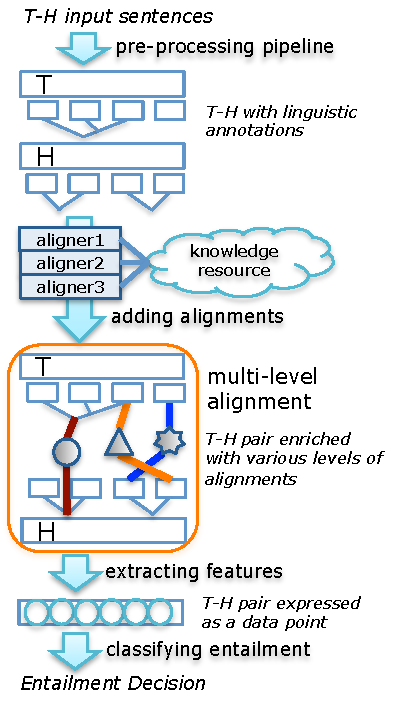
\includegraphics[width=0.8\columnwidth]{figures/figure1.pdf}
  \caption{Dataflow of the proposed approach}
  \label{fig:1}
\end{figure}

(Explanation of the figure - flow down) 

(Two major differences) 
(- no alignment selection: various levels of alignments co-existing in
this layer. no one alignment is the correct one. ) 
(- alignments as main internal representation. traditionally,
knowledge resources and algorithm modules were called from core
algorithm, however, here, all processings before feature extraction
are  )


\section{Implementation and Evaluation (1.5 page)}
What we report in this paper is a pilot study testing the potential of
the proposed architecture. This section first describes the
implementation detail such as pre-processing pipelines, knowledge
resources, aligners and features. 

And the section concludes with the evaluation result of the system on
RTE and application data-set.   

\subsection{Pre-processing, knowledge components, and data representation} 
We used an open source TE platform \cite{EOP-demo} as the supporting
tool for this implementation. The platform provides various
multilingual pre-processing pipelines, and also provides knowledge  
resources wrapped in a standardized manner for our target languages.
Among the available set of multilingual pre-processing pipelines, we
have used Maltparser with TreeTagger, for all three target languages
English, German and Italian. The platform also provides common
interface access for various lexical resources, and all knowledge
resources used with the lexical aligner are accessed via this
interface. 

Another important service that is provided by the platform is the
capability of representing complex data types in a common data
representation. This naturally includes normal linguistic annotations
(such as POS, lemma, parse tree, NER...), but this also includes the
ability to present alignment between any annotation. It permit us to
represent well-known alignments over words and phrases, but also
between parse-trees, NERs, and between any annotations added to T-H
side. This enabled us to define a multilingual ``multi-level
alignment''  representation layer, with minimal new data type
definitions.
%The representation of the platform
%is based on UIMA CAS, and requires some learning curve to represent
%the data, but this enable us to embed one common alignment
%representation layer for ``any future'' alignments.  
By utilizing those existing modules of a common platform, we were able
to concentrate on the core-algorithm implementations.   

\subsection{The (minimal) aligners}
For this pilot study, we have used two main aligners. One is lexical
aligner that connects possible (local) relations based on lexical
resources.

(lexical aligner works via lexical resource, add links that means this
two are related locally. all links has directions, according to the
lexical resources. Each resource become one aligner that links lemmas)

(Phrase aligner, difference, surface level (tokens).)  

(Both lexical and phrase aligner requires scan phase of T-H. We
implemented a linear time look up routine.)

Note that, the aligners connected here are really minimal, and
language independent in this study. Developing and using more
sophisticated aligners for each language is future work of our study.

\subsection{The (minimal, language independent) features} 



\subsection{Experimental results} 
RTE3 was one of the evaluation workshop for TE. It has 800 training
and 800 testing T-H pairs, and later it was translated to both German
and Italian. The following table shows the 


(Entailment Graph making)


\section{Conclusion (0.5 page)} 
   %% * Results: it works! May not be as good as best alignment-based systems
   %%   BUT is extensible, robust, and multilingual
   %% * AND it is available and anyone can use it, not some research prototype (!!!

   Cite.. \cite{Katz:1987}.

%% \section*{Acknowledgments}

%% Do not number the acknowledgment section.
\bibliographystyle{naaclhlt2015}
\bibliography{sem2015_short}

\end{document}
